\chapter{The CMS experiment}
\label{chap:cms}
\chapterquote{You need something to open up a new door, \\
To show you something you seen before, \\
But overlooked a hundred times or more.}
{Bob Dylan}

\section{The LHC}

The \LHC is an octagonal 27km ring (large) proton-proton (hadron) particle collider. Using a multistage acceleration process two beams of protons are circulated in opposite directions at a centre-of-mass energy, $\sqrt{s}$=7~TeV (8~TeV) for data collection in 2011 (2012). The beams of protons are accelerated and circulated by electric and magnetic fields respectively. Further precision magnetic fields can control the position and intensity of the beams. There are four points around the ring where the beams can be forced to intersect producing high energy proton-proton collisions. Particle detectors are constructed around these points such that the collision can be reconstructed with the purpose of measuring physical properties and processes, calibrating the detectors with already known processes and searching for new physics. The remainder of this chapter concentrates on a description of one of these detectors, the \CMS, which the author has worked on.

\section{The CMS detector}

The \CMS detector, pictured in Fig.~\ref{fig:cms_diagram}, is a multipurpose experiment designed for the measurement of and search for a multitude of different processes. We will primarily discuss its function as a Higgs finding machine, a more detailed description can be found in Ref.~\cite{CMS_JINST}. It has a cylindrical shape consisting of a barrel segment, 21.6m long, and two endcaps, 14.6m in diameter, aligned along the beam direction with its centre at the beam interaction point. The endcaps are those nearer the beam line and so the materials in these components typically have to be able to withstand higher amounts of radiation and therefore tend to have worse performance. Many of its features exploit what one would expect for measuring Higgs decays: it has almost full coverage of the area around the collision point so that nearly every particle emanating from the collision can be reconstructed, it has many complimentary subsystems (or layers) designed to measure different specific particles so that Higgs bosons can be detected through a multitude of decay modes. 

For a Higgs with an intermediate mass (100 - 200 \GeV) the high resolution (narrow peak) channels are \HZZ \footnote{A * denotes that one $Z$ can be off mass shell} and \Hgg so good energy resolution and identification of electrons and muons is desirable down to very low \pT ($\sim O(10$\GeV) as well as good resolution and identification of high energy photons. 

The central design feature of \CMS is the very powerful superconducting magnet which produces an axial magnetic field of 4T. The size of this field, as well as the density of the calorimeter materials, allows for a compact and economical design (much more so than its sister detector, ATLAS). Outside of the magnet lie the muon stations which also serve as a return yoke for the magnetic field. The muon chambers in the barrel consist of alternating layers of drift tubes and restive plate chambers which provide both accurate timing and hit location, in order to reconstruct muons down to low energies. In the endcap the drift tubes are replaced with cathode strip chambers. Combining information from the muon subsystem with information from the inner tracking system (described below) allows muons at \CMS to be reconstructed down to $p_{T}<10$~GeV with a resolution of $\sim1\%$. The other three main subsystems at \CMS, the tracking system and the calorimeters, are located inside the magnetic field.

The first layer is the tracking system which is used to reconstruct the momentum of any outgoing charged particles and to locate the primary and secondary vertices. This is surrounded by the calorimeters, the \ECAL and the \HCAL. The first is a single layer of dense, transparent crystals which collects deposits of energy left by electrons and photons which shower inside the material. The second compliments this by providing a measurement of the energy deposited by hadrons (reconstructed as objects known as jets) through nuclear interactions. The \HCAL is a sampling calorimeter in which the active material (plastic scintillator) is sandwiched between a dense absorbent material (brass or steel). This extends the radiation length of the calorimeter (clearly accommodating the compact design) and provides pointing information but degrades the resolution of reconstructing jets. 

\CMS uses a right-handed Cartesian coordinate system with the origin at the interaction point and the $z$-axis pointing along the beam axis. The $x$-axis points towards the centre of the \LHC ring and the $y$-axis points vertically upwards. The azimuthal angle, $\phi \in [-\pi,\pi]$, is defined with respect to the $x$-axis in the transverse $(x-y)$ plane. The polar angle $\theta$ is measured from the $z$-axis. Commonly, the direction of an outgoing particle is defined by $\phi$ and its pseudo-rapidity $\eta$,

\begin{equation}
	\eta = -\ln\tan\biggl(\frac{\theta}{2}\biggr).
\end{equation}

The \LHC is capable of producing 40M bunch collisions per second although many of these are not hard interactions, the result being that the outgoing particle debris follows the beam line. A hard (and therefore interesting) collision is characterised by the amount of energy produced in the transverse ($x-y$) plane. Therefore particles are commonly characterised by the projection of their momentum onto this plane, their transverse momentum,

\begin{equation}
	p_{T} = \sqrt{p_{x}^{2}+p_{y}^{2}},
\end{equation}

and the corresponding transverse energy, $E_{T} = E\sin(\theta)$.

\begin{figure}
  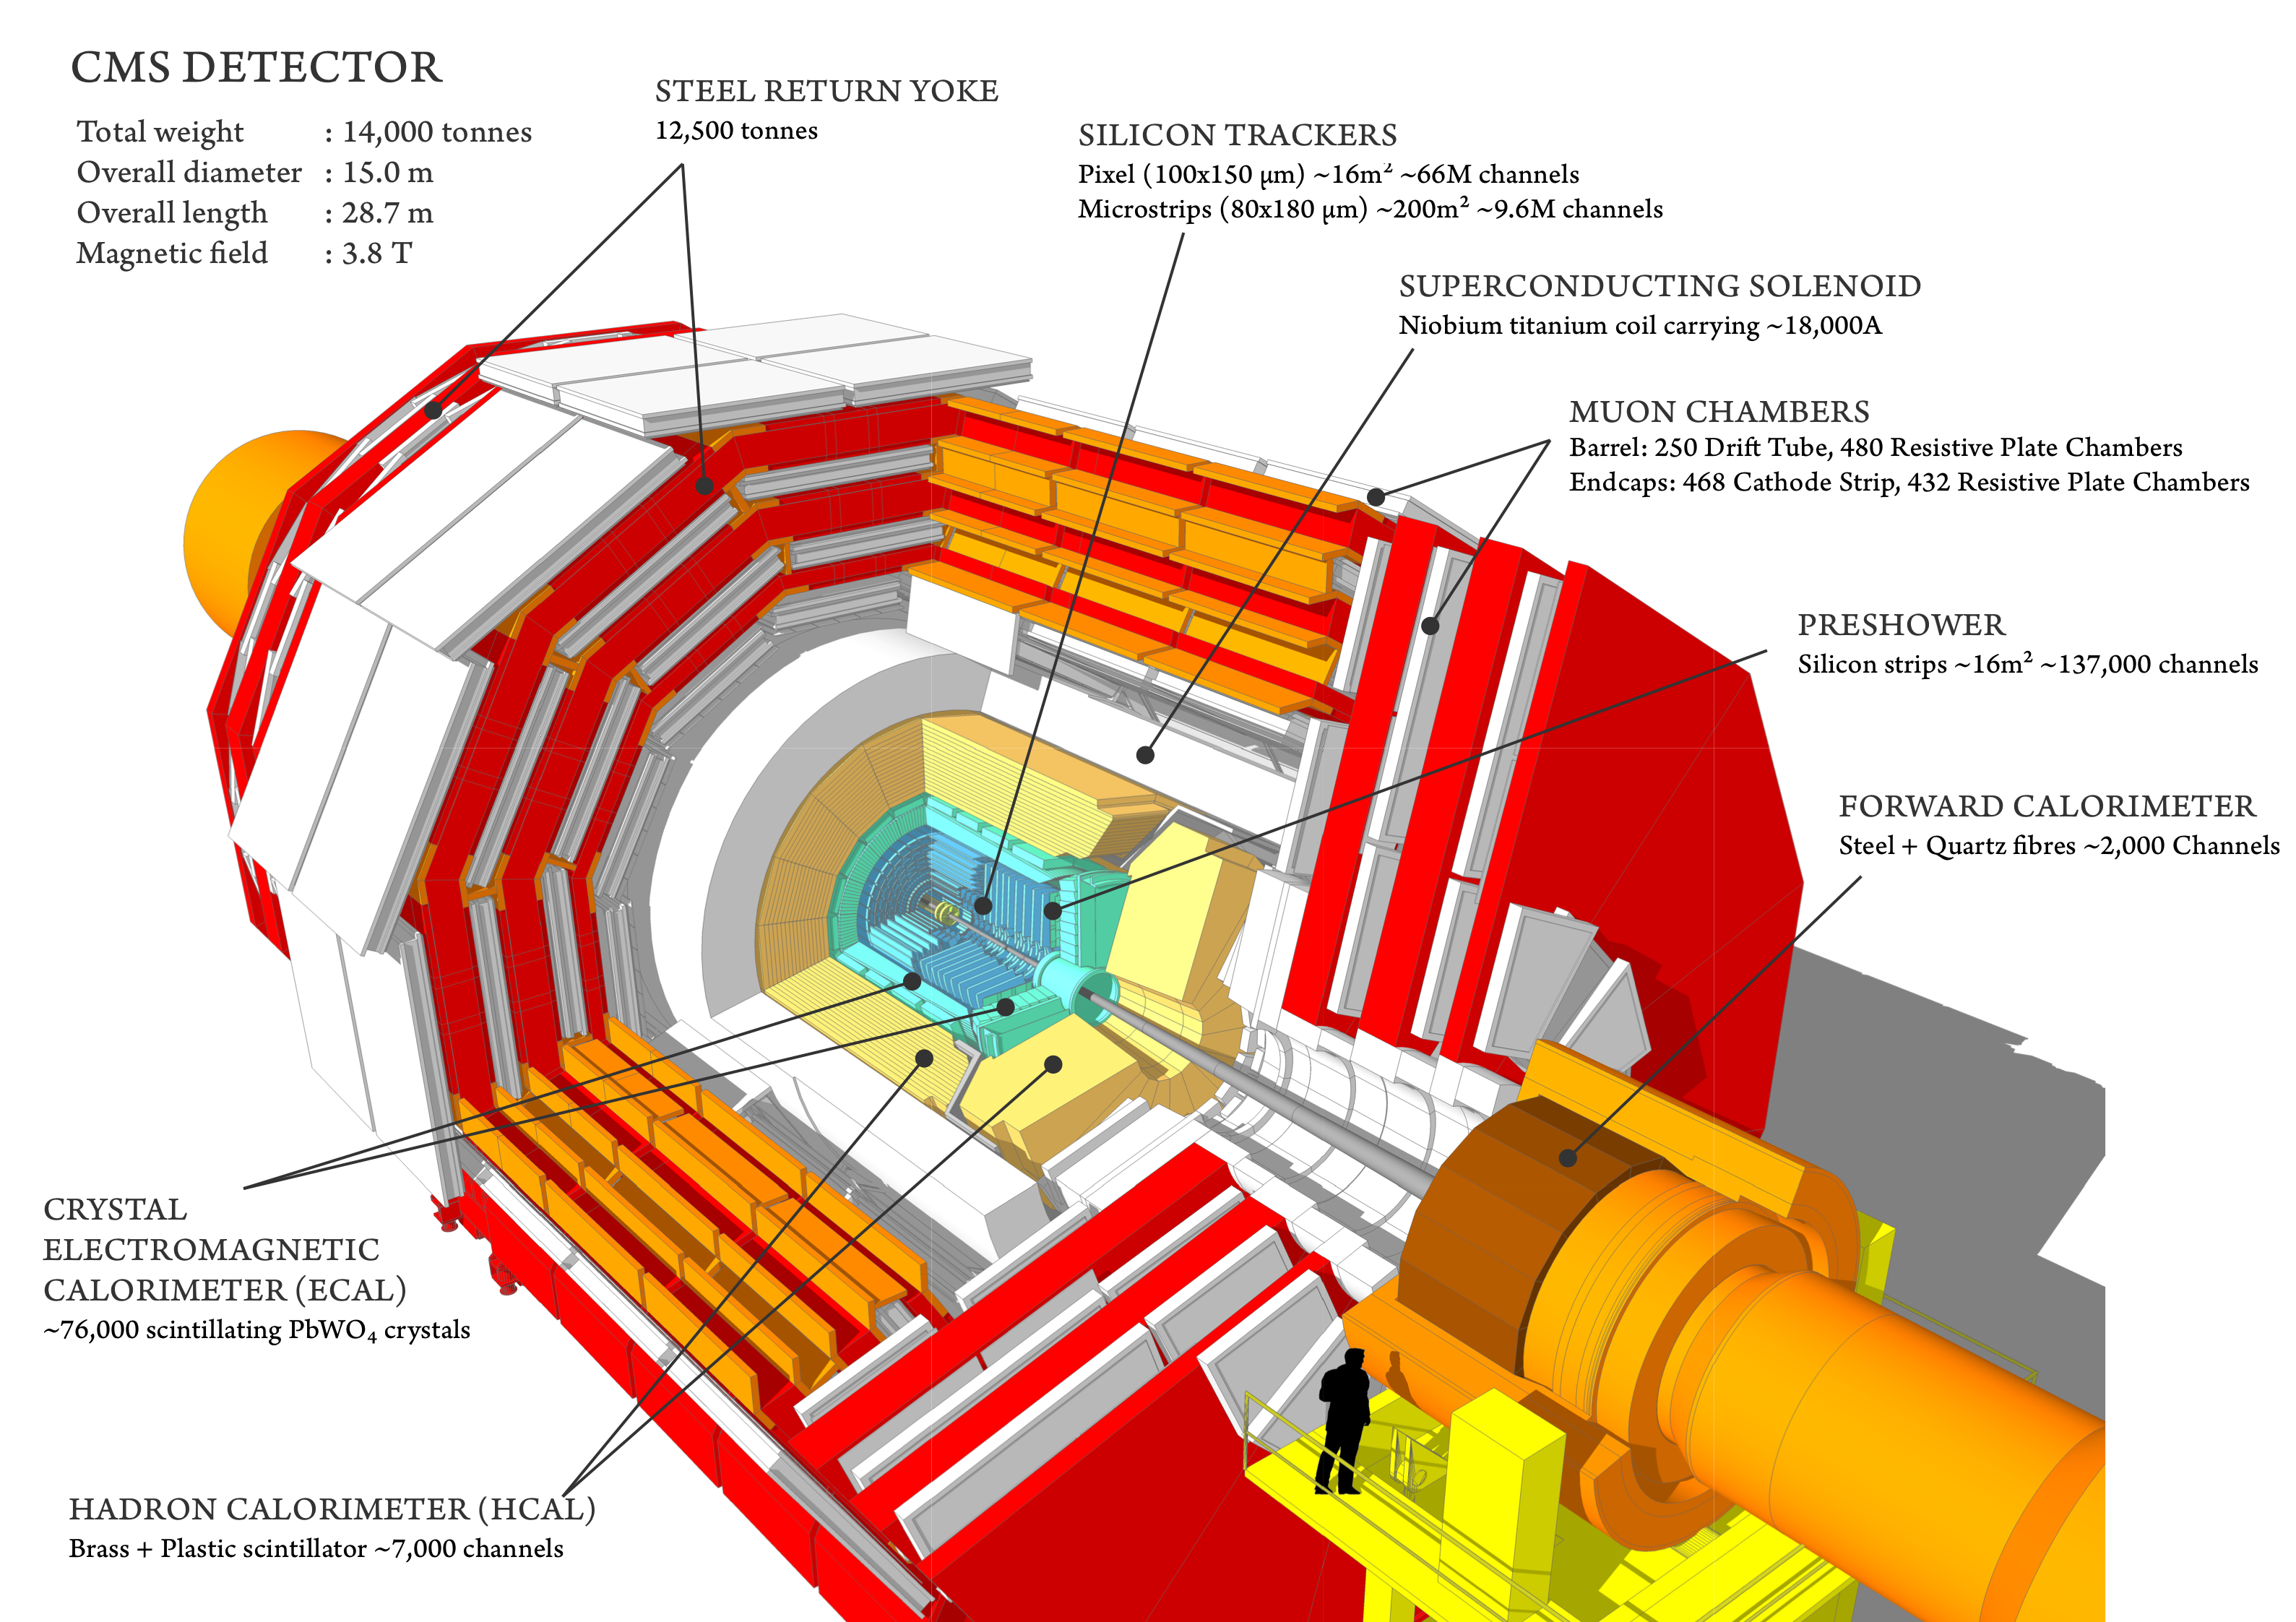
\includegraphics[width=0.8\textwidth]{ch2_cms_exp/plots/cms_diagram.png}
  \caption[CMS diagram]{This is a schematic representation of \CMS showing the layered structure of subdetectors; tracking system, calorimeters, magnet and muon system.}
  \label{fig:cms_diagram}
\end{figure}

% --------- TRACKER ----------
\subsection{Tracking system}
\label{sec:tracker}

During nominal \LHC running conditions in 2012 there on average over 1000 particles from up to 50 overlapping \pp collisions (pileup) per bunch crossing (every 50 ns). The tracker is designed to efficiently and precisely reconstruct all charged particle trajectories, thus their position and momentum, which are known as tracks. Due to the vast number of tracks eminating from multiple vertices in typical \LHC collisions the tracking material and electronics are required to have high granularity, a fast response and be radiation hard. This conflicts with another important design feature of the tracker which is the aspiration to use the minimal amount of material in order to reduce multiple scattering, bremsstrahlung, photon conversion and nuclear interactions before particles reach the calorimeters. These criteria motivate the choice of silicon throughout the \CMS tracking system. The structure of the \CMS tracker is shown in Figure~\ref{fig:cms_tracker} and consists of a central pixel detector surrounded by layers of silicon strips aligned parallel to the beam line in the barrel (TIB and TOB) and perpendicular to the beam line in the endcap (TID and TEC).

By making multiple precise measurements of tracks as they pass through the pixel and silicon layers (hits) the track trajectory can be reconstrcuted and their momentum calculated using their curvature in the \phi plane due to the axial magentic field. Tracks are grouped together (requiring that their separtion is less than 1cm in the $z$ coordinate at the point of closest approach to the beamline) and assigned to a common point or origin (the primary vertex). The vertex resolution is driven both by the number of tracks originating from a particular vertex and how large their average \pT is. This is shown in Fig.~\ref{fig:tracker_vertex_resolution} for preliminary data taken in 2010 at $\sqrt{s}=7$~TeV.

\begin{figure}
  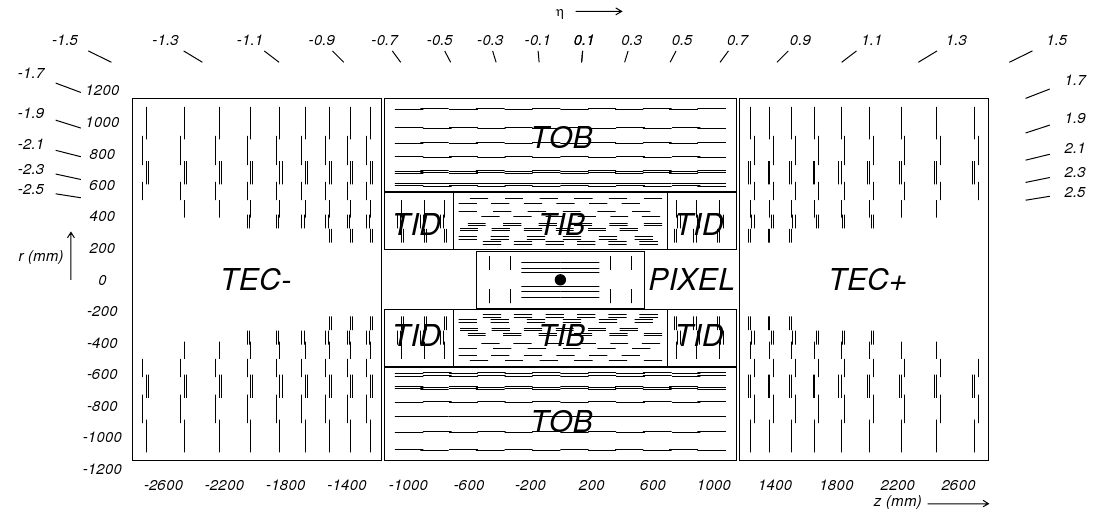
\includegraphics[width=0.9\textwidth]{ch2_cms_exp/plots/fig_cmstracker.png}
  \caption[CMS tracker]{A diagram of the \CMS tracking system showing the PIXEL detector and outer silicon strip layers~\cite{CMS_JINST}.}
  \label{fig:cms_tracker}
\end{figure}

\begin{figure}
  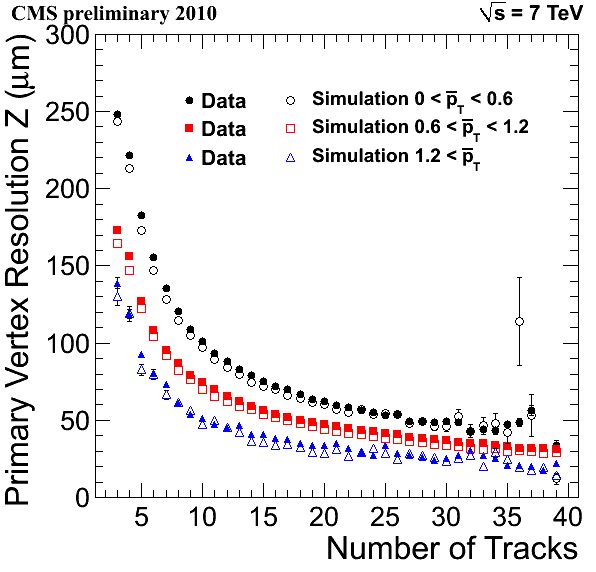
\includegraphics[width=0.48\textwidth]{ch2_cms_exp/plots/ResZ_byPt.png}
  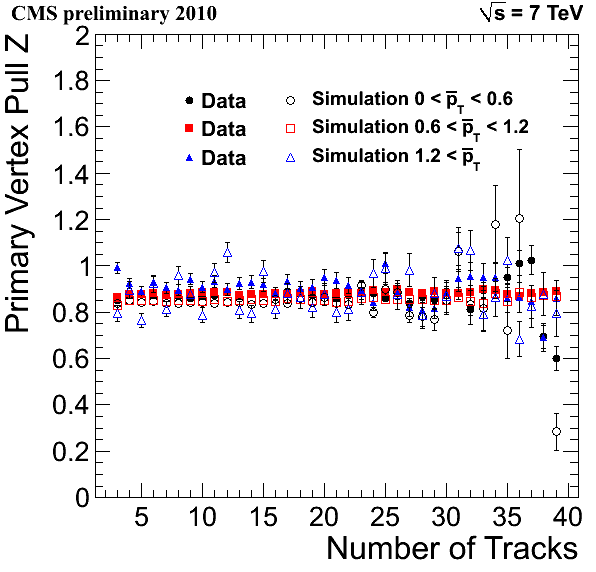
\includegraphics[width=0.48\textwidth]{ch2_cms_exp/plots/PullZ_byPt.png}
  \caption[Vertex resolution]{A demonstration of the vertex position resolution in Z as a function of the number of tracks originating from that vertex. The different colors respresent three different bins in the average track \pT where data is shown as solid points and simulation as open points~\cite{cms-tracker-performance-2010} }
  \label{fig:tracker_vertex_resolution}
\end{figure}

The material budget for the tracker is shown in Fig.~\ref{fig:tracker_material} which demonstrates as a function of \eta which subsystems of the tracker, beam pipe and servicing contrubute to material inbetween the interaction point and the calorimeters in radiation lengths (X$_{0}$) and nuclear interaction lengths ($\lambda_{I}$). As shown in Fig.~\ref{fig:cms_tracker} the tracker has full coverage in \phi and up to $|\eta|\leq2.5$. As we will see later the tracking system is very important for the \Hgg search at \CMS as without it locating the primary vertex would be practically impossible.

\begin{figure}
  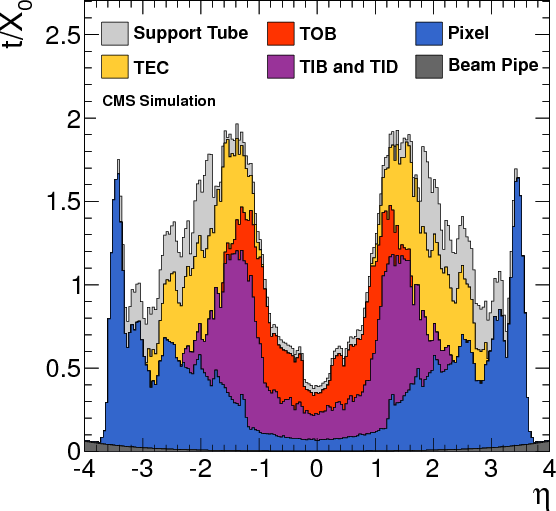
\includegraphics[width=0.48\textwidth]{ch2_cms_exp/plots/tracker_material.png}
  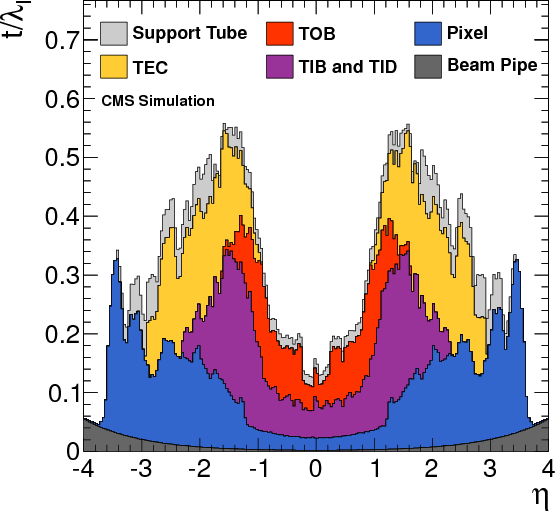
\includegraphics[width=0.48\textwidth]{ch2_cms_exp/plots/tracker_material_lambda.png}
  \caption[CMS tracker material budget]{The amount of \CMS tracker material in radiation lengths (X$_{0}$) on the left and in nuclear interaction lengths ($\lambda_{I}$) on the right as a function of $\eta$ for the different tracking subsytems.}
  \label{fig:tracker_material}
\end{figure}

% --------- ECAL SECTION ----------
\subsection{Electromagnetic calorimeter}
\label{sec:ecal}

The \ECAL is used to reconstruct the energy of electrons and photons which deposit their energy via electromagnetic showers inside the calorimeter material. The shower inside the crystal produces photons whose total energy is proportional to the energy of the incoming particle, hence the light output from the shower can be measured by photodiodes at the back of each crystal which in turn provides a measurement for the energy of the original particle. The \ECAL has full hermetic coverage of the interaction point and consists of a single layer of \PbWO crystals. The crystals are laid out in a quasi-projective geometry such that they point towards the interaction point with an offset of 3$\degree$ making it much less likely that a photon, or electron, will pass straight through a gap between crystals. The \ECAL consists of a barrel section and two endcap disks which are preceded by a preshower (to aid with \pizero rejection), a schematic is shown in Fig.~\ref{fig:cms_ecal}. There is a fiducial region between the barrel and endcap (to prevent reconstruction of showers which overlap both subsystems) yielding an \ECAL coverage of $|\eta|<2.5$ but not in the range $1.444<|\eta|<1.556$ and full coveraege in \phi. The crystals in both sections have a depth of 23cm (which amounts to 25.8~X$_{0}$) implying that practically the whole depth of the shower is contained within this single layer. 

\begin{figure}
  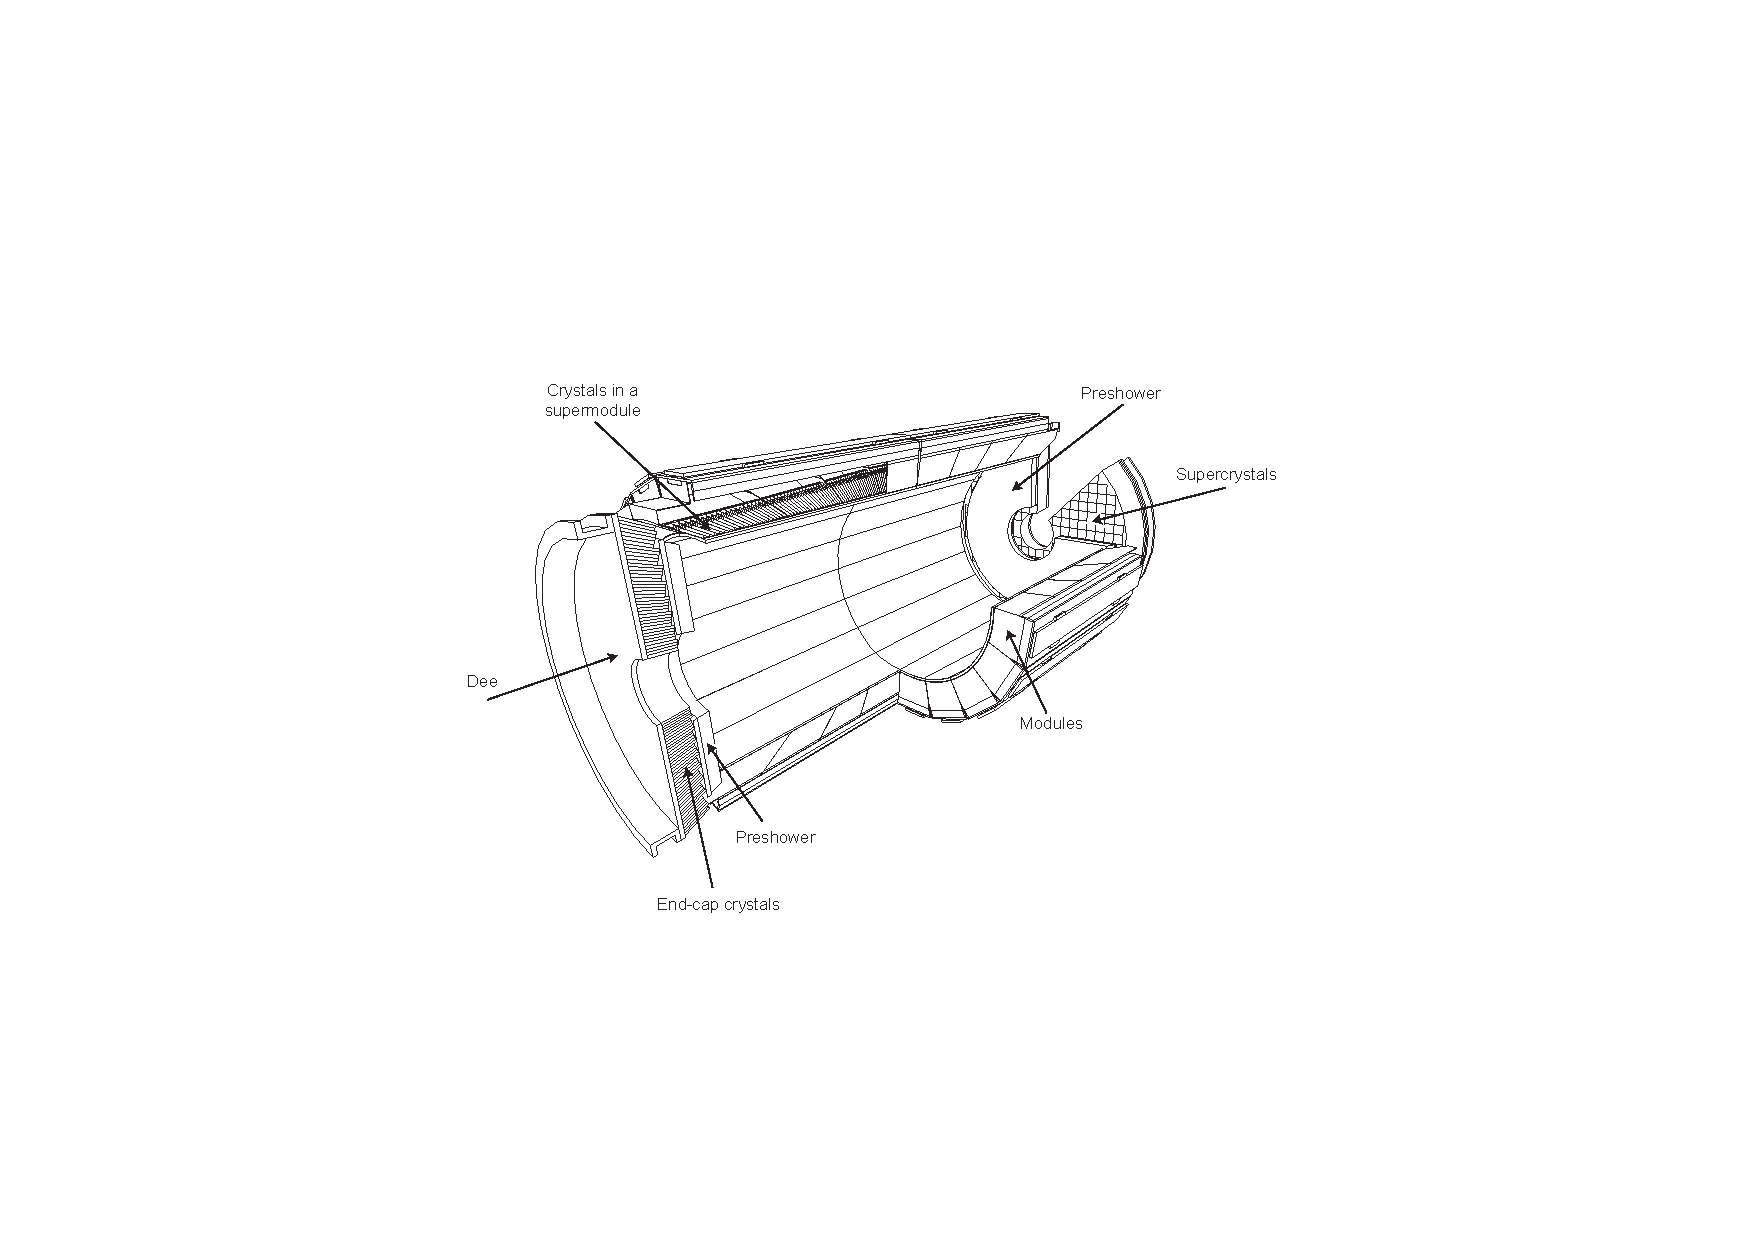
\includegraphics[width=0.7\textwidth]{ch2_cms_exp/plots/cmsecal.pdf}
  \caption[CMS ECAL schematic]{A schematic drawing of the \CMS \ECAL layout showing the ``modules" of crystals in the \ECAL barrel and the "Dees" of crystals in the \ECAL endcap~\cite{CMS_JINST}.}
  \label{fig:cms_ecal}
\end{figure}

\PbWO has some attractive properties for an electromagnetic calorimeter especially when considering \Hgg decays. In order to acheive good energy resolution it is desirable to have a design in which most of the electromagentic shower from an incoming photon or electron is contained within a single crystal, as less of the shower (and therefore energy) is lost in cracks and gaps inbetween crystals. \PbWO has a short radiation length ($X_{0}=0.89$cm) which compliments a compact design as the entire depth of the shower can be contained in a crystal which is not very long. It has a small Moli\`{e}re radius (1.96cm) which means that the lateral size of the shower is small. This generally means that the cross-sectional size of a crystal can be small (yielding high granularity of the detector) whilst still containing a large percentage of the shower. It has a very short scintillation time decay constant (85\% of the light is collected in 25ns), in other words it is very ``fast", allowing the energy in the shower to be collected and measured very quickly. This is clearly desirable in an environment like the \LHC when collisions are happening up to every 25ns. The one draw back of \PbWO (apart from expense) which has crippled its use in detectors previously is its incredibly low light yield at room temperature ($\sim$50-80 photons/MeV). This is overcome at \CMS with the use of silicon \APDs in the ECAL barrel and \VPTs in the endcap, which amplify the signal enough to make accurate measurements of the original photons energy. 

\subsubsection{Energy resolution}

As we have seen previously (\red{assume this formula will appear in the Introduction and can be referenced}) the diphoton invariant mass is given by,

\begin{equation}
  m_{\gamma\gamma} = \sqrt{2E_{1}E_{2}(1-\cos\alpha)},
  \label{eq:dipho_inv_mass}
\end{equation}

where $E_{1}$ and $E_{2}$ are the energy of the two photons and $\alpha$ is the angle between them. Therefore the mass resolution has terms that depend on the photon energy resolution and angular resolution,

\begin{equation}
  \frac{\sigma_{M}}{M} = \frac{1}{2} \Biggl[ \frac{\sigma_{E_{1}}}{E_{1}} \oplus \frac{\sigma_{E_{2}}}{E_{2}} \oplus \frac{\sigma_{\alpha}}{\tan(\alpha/2)} \Biggr],
  \label{eq:mass_res}
\end{equation}

where $\sigma$ denotes the resolution and $\oplus$ the quadratic sum. It is therefore desirable to have both good energy resolution and good position resolution for photons (accurate position measurements at the \ECAL face alongside knowledge of the primary vertex can be used to calculate the individual photons' direction and ergo the angle between them). The energy resolution is usually then further parametrised as,

\begin{equation}
  \frac{\sigma_{E}}{E} = \frac{a}{\sqrt{E}} \oplus \frac{b}{E} \oplus c,
  \label{eq:energy_res}
\end{equation}

where $a$ is the stochastic term, $b$ the noise term and $c$ a constant term. In order to acheive the best possible resolution all three of these terms need to be of a similar order and as small as possible. The size of these terms has been determined from test beam data in Ref.~\cite{CMS_JINST}. The stochastic term is driven by the material choice and detector type so cannot be improved once the machine is built. The main contributions to this term are lateral shower containment fluctuations, photostatistics and fluctuations in the energy deposited in the preshower absorber. For a fully active calorimeter (the \CMS \ECAL is not a sampling calorimeter) made of \PbWO the size of this term is good ($a=2.8\pm0.3\% $GeV$^{\frac{1}{2}}$). The constant term, which depends on non-uniformity of longitudal light, intercalibration errors and energy leakage from the back of the crystal, can be minimzed by use of \emph{in situ} calibration of individual crystals and amounts to $c=0.26\pm0.05\%$. However the \Hgg analysis at \CMS dispenses with the intercalibration constants by using a regression technique to estimate the photon energy which is discussed in Section~\ref{sec:photon_energy}. The noise term which has contributions from electronics noise (including signal digitisation) and event pile-up (additional particles causing overlapping signals) is measured as $b=126$MeV. The ECAL energy resolution, $\sigma_{E}/E$, as a function of electron energy is shown in Fig.~\ref{fig:sigma_e_test_beam} as measured from a beam test. 

\begin{figure}
  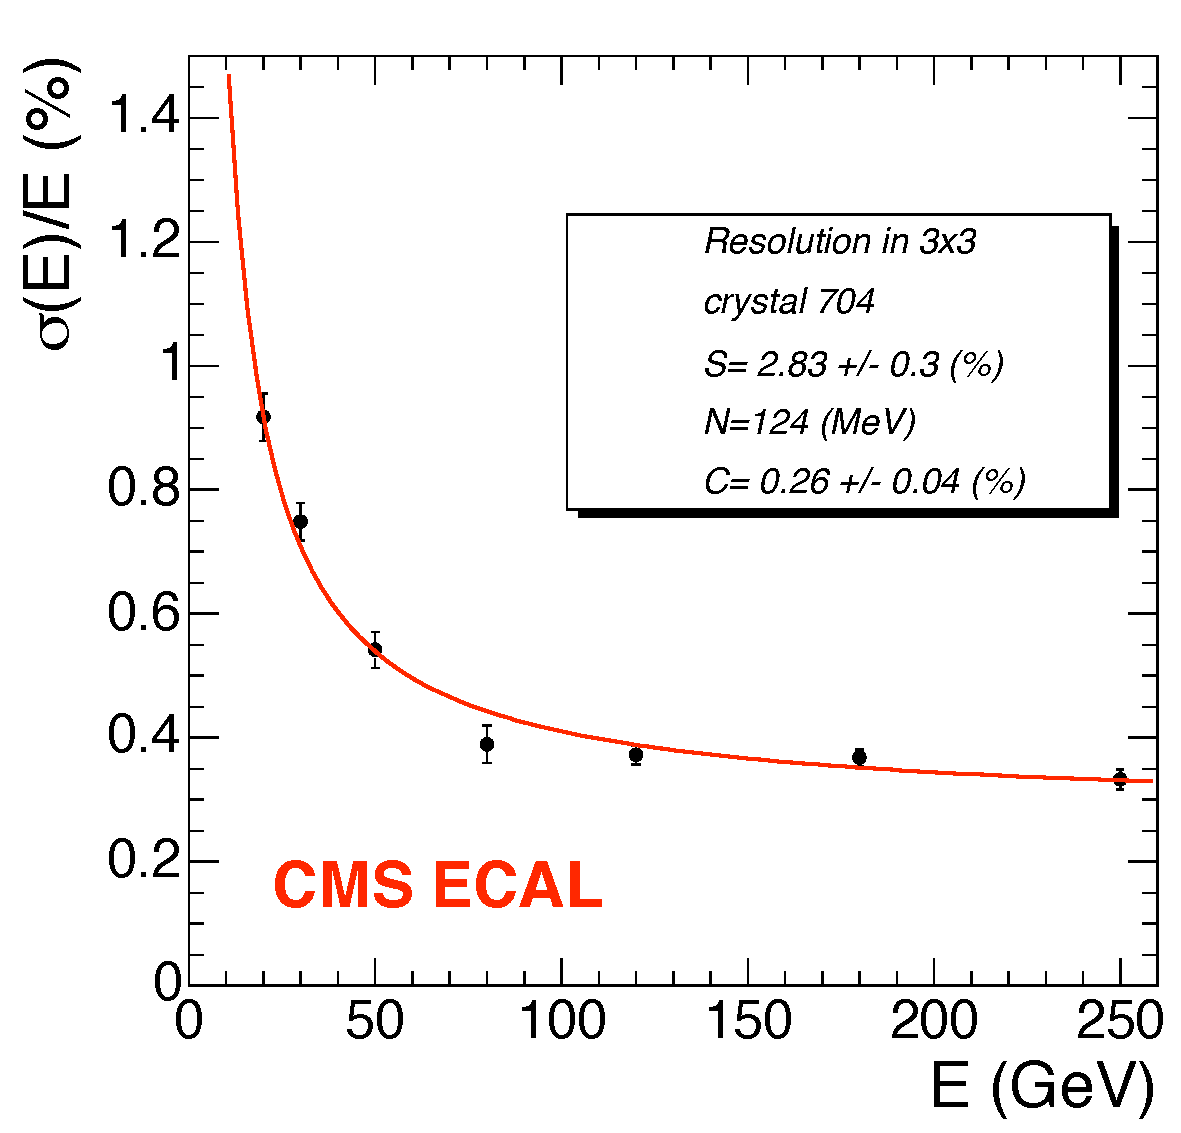
\includegraphics[width=0.6\textwidth]{ch2_cms_exp/plots/ecal_sigma_e_test_beam.pdf}
  \caption[ECAL energy resolution]{The \ECAL energy resolution, $\sigma_{E}/E$, as a function of electron energy measured from test beam data. The energy is measured in a 3$\times$3 array of crystals centered on crystal of electron impact~\cite{CMS_JINST}.}
  \label{fig:sigma_e_test_beam}
\end{figure}

\subsubsection{Transparency corrections}

Due to the high particle flux present at \CMS the \ECAL crystals and electronics have to be radiation hard, especially in the endcap. This is another motivating factor for using \PbWO as the crystal material. The crystals are additionally doped with Nb to improve the induced absorbtion coefficient. Over time and long exposure to radiation the crystals loose their transparency, although there is considerable natural recovery during down periods. An important part of the \ECAL monitoring and calibration comes in the form of transparency corrections to compensate for these losses. At regular intervals during \LHC running laser pulses are injected into the crystals to measure the crystal response. Two different wavelengths of laser are used, one blue ($\lambda=440$nm) which is very similar to the scintillation emission peak and therefore expected to be affected by transparency changes in a similar way to typical scinitillation light, and one red ($\lambda=796$nm) which is far from the scinitillation emission peak and affected very little by the changes in transparency. Hence, by comparing the red and blue laser light response, time and $\eta$ dependent corrections for crystal transparency loss can be calculated. A closure test for these corrections, in 2012 data, is shown in Fig.~\ref{fig:ecal_laser_corrs} which shows the ratio of electron energy (calculated from the \ECAL) to electron momentum (calculated from the tracker) before and after transparency (or laser) corrections. 

\begin{figure}
  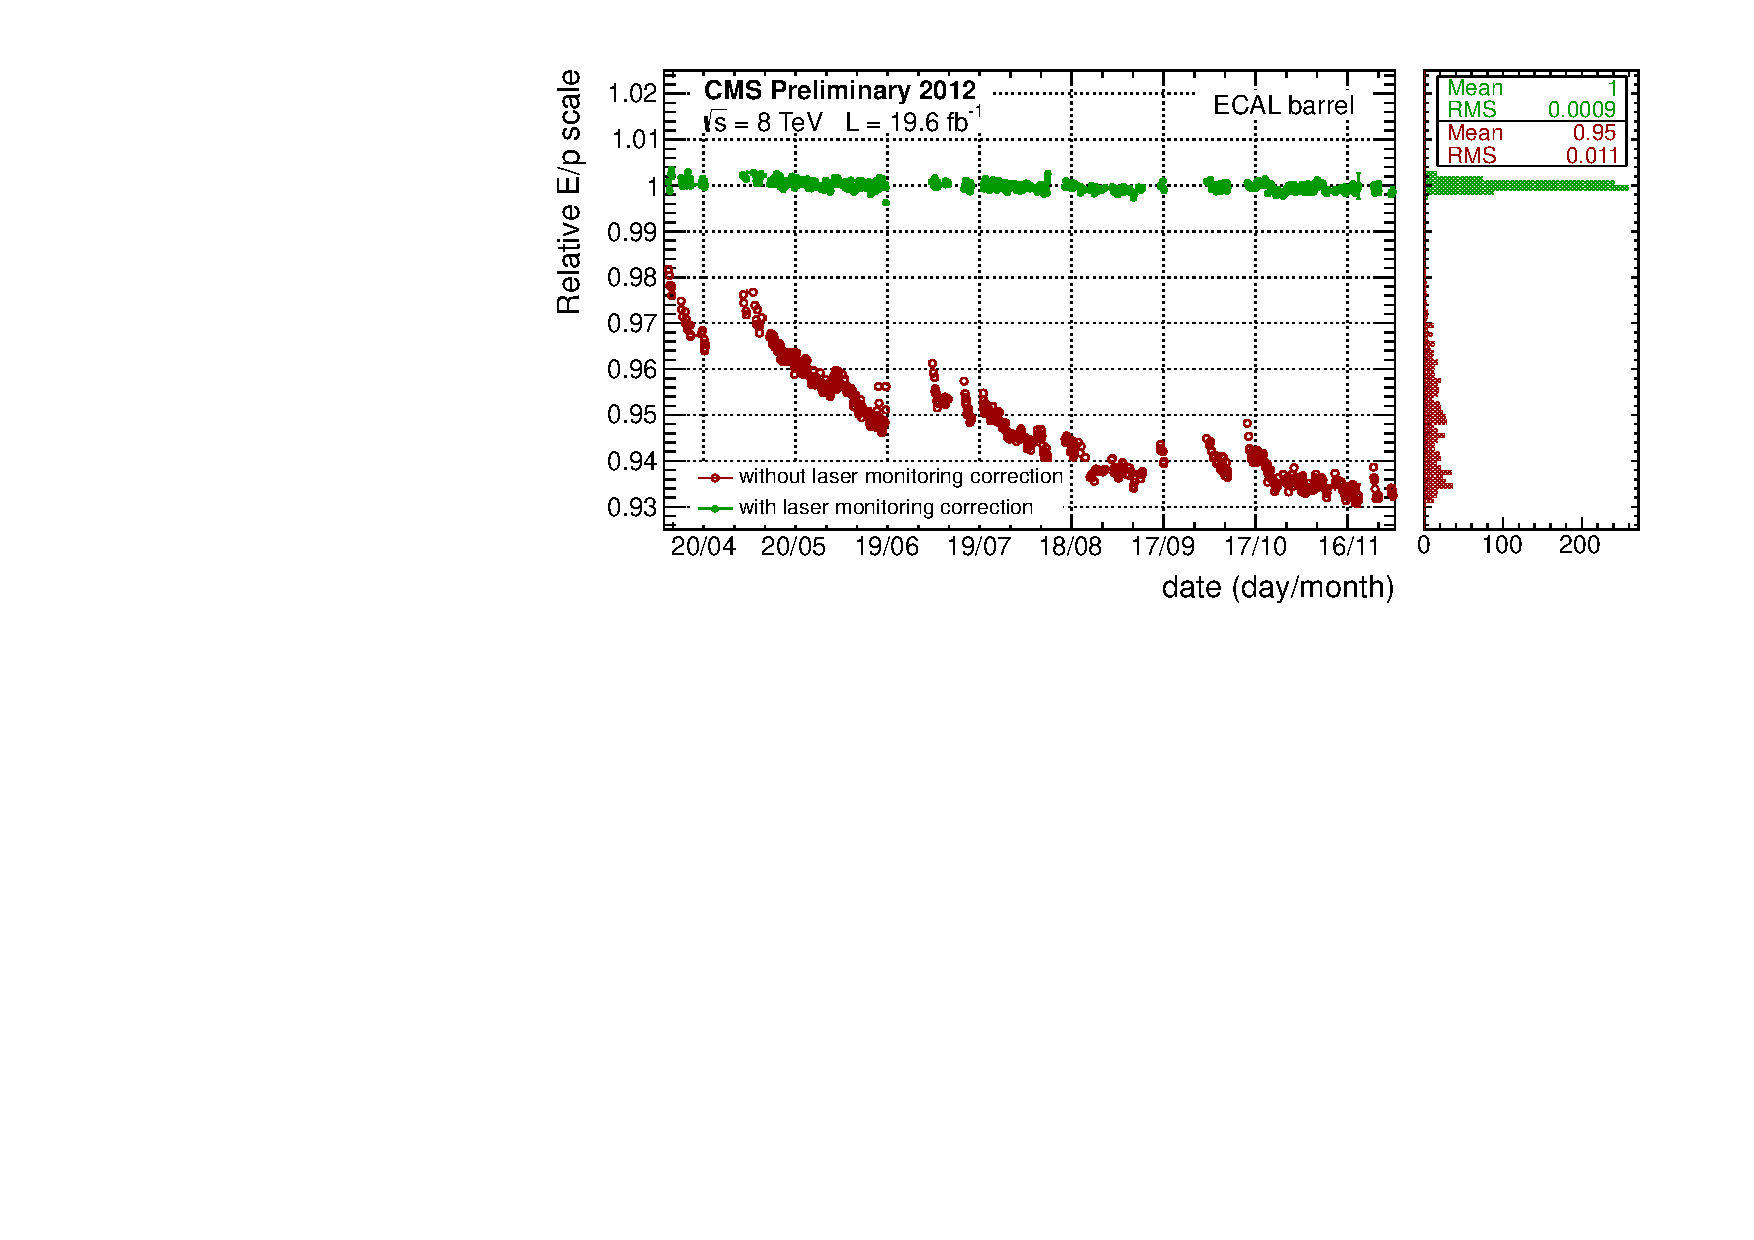
\includegraphics[width=\textwidth]{ch2_cms_exp/plots/ecal_EB_lasercorrs.pdf} \\
  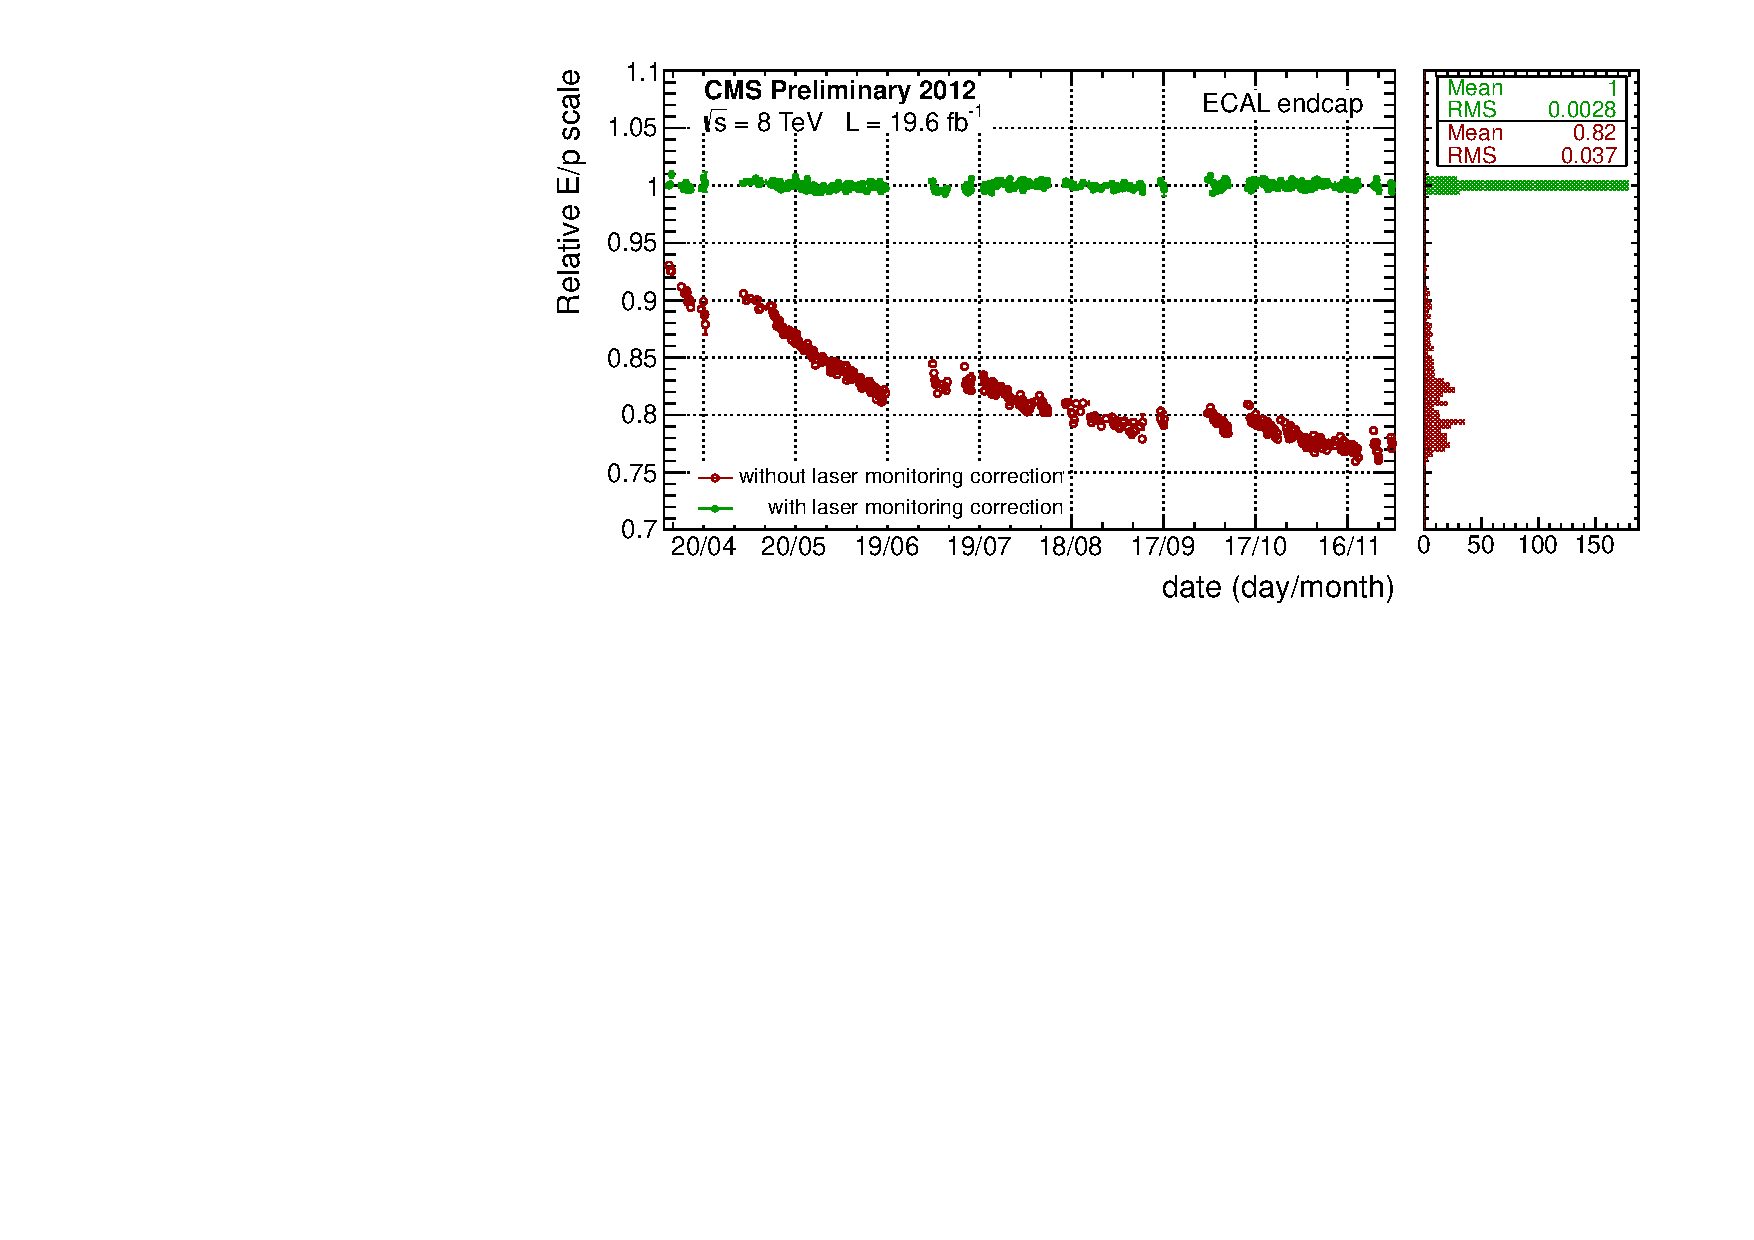
\includegraphics[width=\textwidth]{ch2_cms_exp/plots/ecal_EE_lasercorrs.pdf} 
  \caption[ECAL laser corrections]{Ratio of the electron energy, $E$, to the electron momentum, $p$, measured in the \CMS barrel (top) and endcap (bottom) for 2012 data. The red (green) points show the performance before (after) the laser monitoring derived corrections ~\cite{cms-ecal-performance-2012}.}
  \label{fig:ecal_laser_corrs}
\end{figure}

\subsubsection{Preshower}

The dominant source of background to high energy photon signals are neutral mesons, mainly pions (\pizero), which decay into two approximately collinear photons and can therefore look very much like a single high energy photon. The \ECAL endcap is preceeded by a preshower to specifically target this and provide the endcap with a higher granularity. The preshower is a sampling calorimeter which consists of two layers: a lead plate, to initiate the shower, in front of a fine grained silicon detector which has two layers of orthogonal strips. There are many other characteristics of \pizero decays which can help in differentiating them from real (``prompt") photons, these include isolation (discussed later in this Chapter in Section~\ref{sec:iso}) and the shower shape (discussed in Chapter~\ref{chap:selection_and_categorisation} in Sections~\ref{sec:cic} and~\ref{sec:mva}).

\subsubsection{Photon reconstruction}

Calculating an incoming photons energy amounts to summing the energy deposited by the electromagentic shower which is initiated by the photon impact at the crystal face. Due to the presence of material in the beam pipe and tracking system (see Fig~\ref{fig:tracker_material}) about 60\% of photons will convert into an electron-positron pair before they reach the \ECAL. If this is the case the shower will spread out in \phi due to the presence of the magnetic field; the photon converts to electrons which bend and Bremsstrauhlung radiate additional photons, and can be distributed among multiple (up to hundreds of) crystals. Consequently clustering (pattern matching) algorithms are deployed to calculate the ``raw" photon energy. Corrections to this energy are subsequently applied to account for any energy loss as explained in Section~\ref{sec:photon_energy}. The shower will appear as a local maxima amongst a spatial neighbourhood of crystal energy deposits and so the algorithms used search first for the most energetic crystals (known as the ``seed" crystals) and then extend to amass as a large a fraction as possible of the original shower energy. There are three cases to include which are i) photons which reach the \ECAL without interacting with any of the intermediate material in the beam pipe and tracking system (referred to as unconverted photons), ii) photons which convert into an electron-positron pair inside the tracker and shower in the barrel, iii) photons which convert and shower in the endcap.

We will first consider the case of converted photons in the barrel. This is so similar to the case of a real electron that the identical algorithm is used for electrons as well. The method used is known as the ``Hybrid" algorithm, depicted in Fig.~\ref{fig:hybrid_algo}, which makes clusters of clusters known as a ``supercluster": a cluster being a set of crystals which pick up an electron or a bremsstraulunged photon and a cluster of clusters being a set of these which make up all the electrons and photons radiated from the original object. The algorithm can be described as a five step process as follows,

\begin{enumerate}
  \item{Locate the seed crystal which is the maximum energy crystal in the search region, not already in a cluster, and which must satisfy the threshold condition, $E_{T}>1$~GeV.}
  \item{Extend in \eta to construct a ``domino" which is 1$\times$3 crystals in $\phi\times\eta$. If the energy of the central crystal in the 1$\times$3 domino is greater than 1~GeV then extend this to a $1\times5$ domino in $\phi\times\eta$.}
  \item{Traverse along \phi, up to a maximum of 17 crystals in both directions, adding dominoes in this way. If a domino has less energy than 0.1~GeV then it is excluded.}
  \item{Of the clusters of adjacent dominoes the seed domino (most energetic) must have energy greater than 0.35~GeV.}
  \item{Repeat starting from Step 1 to build a new supercluster.}
\end{enumerate}

In this way a collection of dominoes are clusted in \phi creating a ``supercluster" of smaller clusters (which has a maximum of area of $5\times35$ in $\eta\times\phi$). A similar but slightly modified algorithm is used for photons and electrons in the endcap. This is known as the ``Multi5$\times$5" algorithm and proceeds,

\begin{enumerate}
  \item{Locate the seed crystal which is the maximum energy crystal in the search region, not already in a cluster, and which must satisfy the threshold condition, $E_{T}>180$~\MeV.}
  \item{The $5\times5$ array of crystals surrounding the seed are summed to make a cluster.}
  \item{Crystals at the edge of the cluster can seed new overlapping $5\times5$ clusters if they are local maxima compared to their neighbouring crystals.}
  \item{Proceed in this way in any direction building an overlapping collection of $5\times5$ clusters to create a supercluster.}
  \item{Repeat starting from Step 1 to build a new supercluster.}
\end{enumerate}

\begin{figure}
  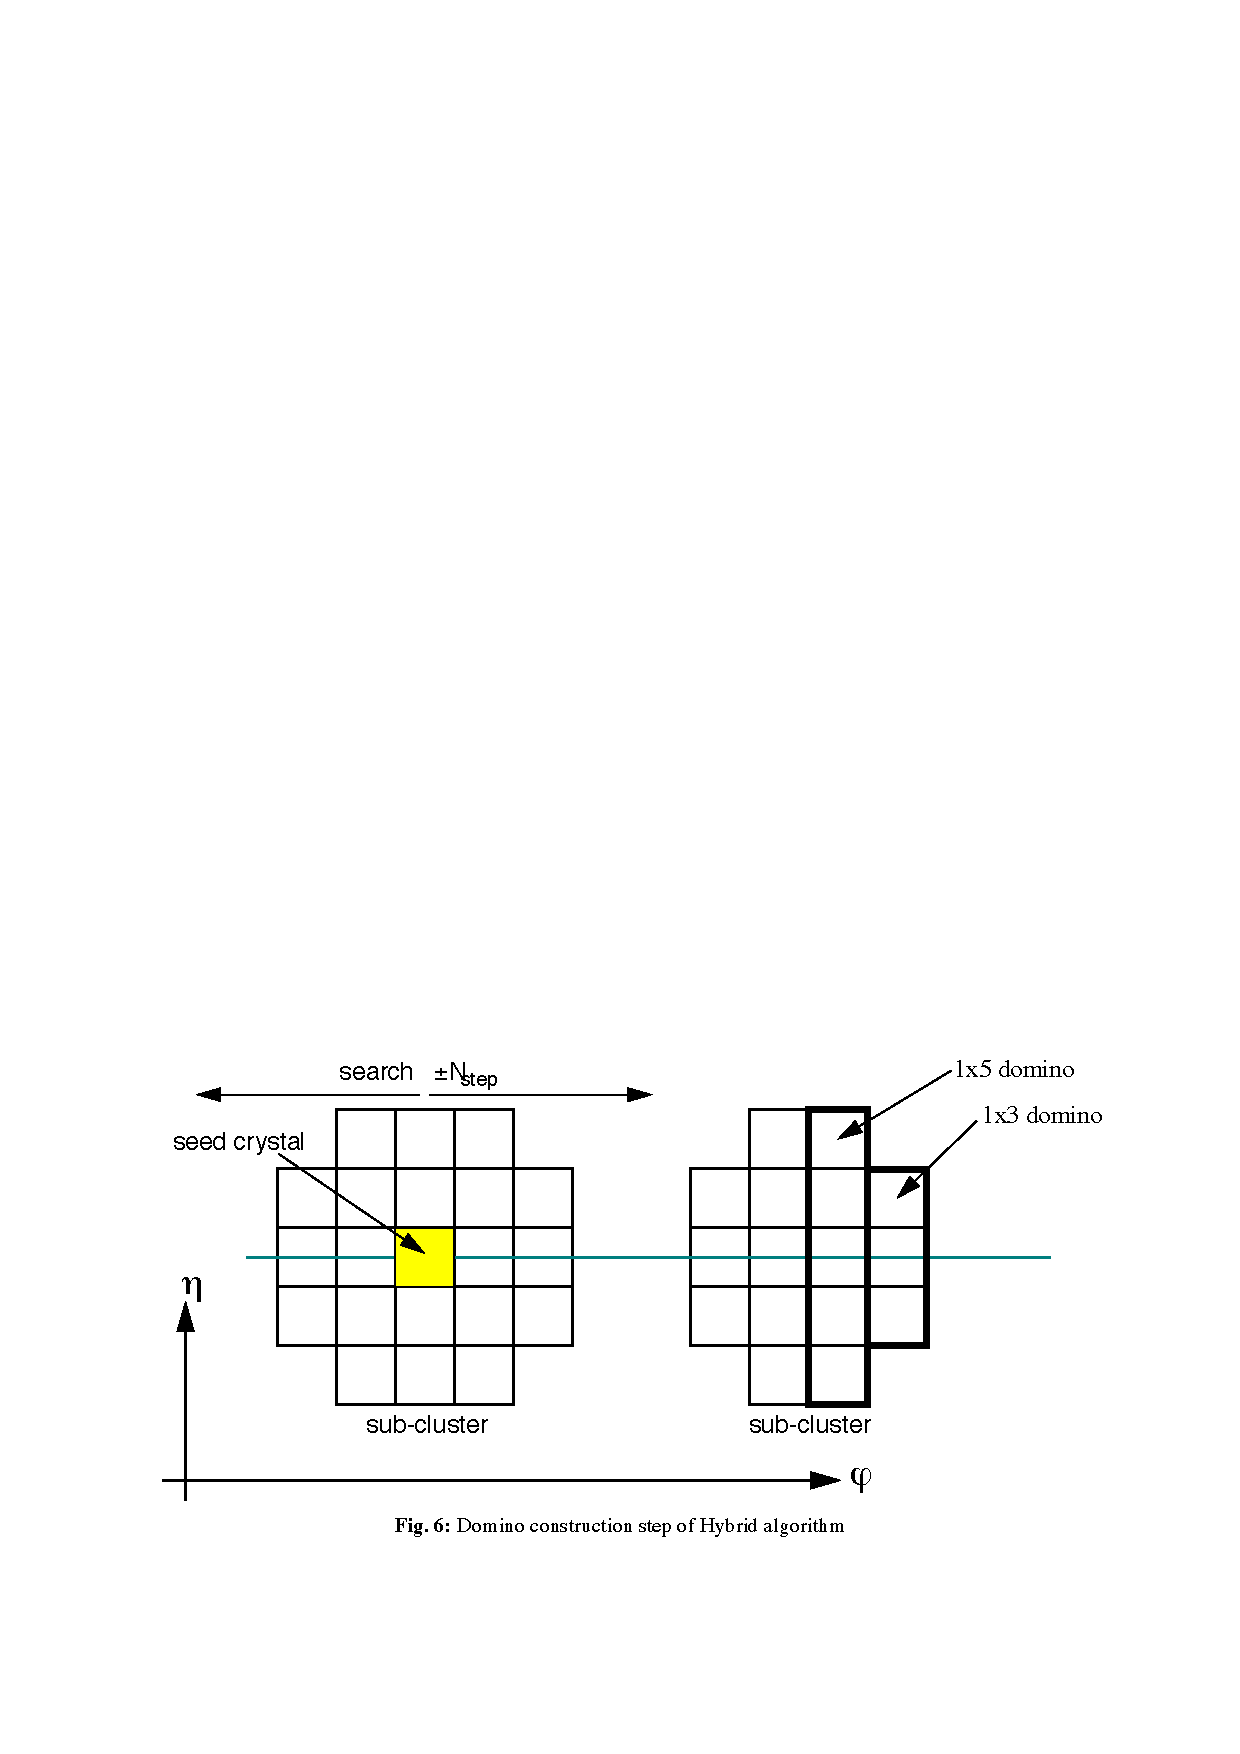
\includegraphics[width=0.8\textwidth]{ch2_cms_exp/plots/hybrid_clustering.pdf}
  \caption{The domino construction setup of the hybrid clustering algorithm~\cite{ecal_electron_reco}.}
  \label{fig:hybrid_algo}
\end{figure}

The final case concerns photons which reach the \ECAL without converting which have a shower that is much more localised in \eta and \phi, about 94\% of its energy is deposited in an area of 3$\times$3 crystals and more than 97\% in an area of 5$\times$5 crystals. This provides a definition for the conversion variable, \rnine, such that, 

\begin{equation}
	R_{9} = \frac{E_{3\times3}}{E_{SC}} 
	\begin{cases}
		\text{unconverted if } R_9\geq0.94 \\
		\text{converted otherwise}.
	\end{cases}
  \label{eq:rnine}
\end{equation}

If a photon fufills the unconverted requirement given above (Eq.~\ref{eq:rnine}) the photon energy is reconstructed as the sum of all energy deposited in the 5$\times$5 array of crystals which surround the most energetic crystal. It has been shown that using a fixed window for non-converting photons yields a better energy resolution than any clustering procedure~\cite{ecal_electron_reco}.

The location of a supercluster is determined as the energy weighted mean position of the crystals in the supercluster. This gives a position resolution which is much smaller than the size of an individual crystal ($\sim20\times20$mm$^{2}$). Values for an electron of \pT=35~GeV in the \ECAL barrel, in the absence of pileup, are $\sigma_{\eta}=1.0\times10^{-3}$, $\sigma_{\phi}=1.6$~mrad.

\subsubsection{Electron and photon differences}

It is clear that when only considering the \ECAL there is no difference between electrons and photons. Consequently at the level of the calorimetry there is no distinction between them, simply the idea of a supercluster which can apply to both. In the case of an electron, information from the tracker can be included using a Gaussian sum filter algorithm~\cite{tracker_electron_reco}, where a series of compatible track hits are associated to the supercluster. This is used to provide a supplementary measurement of the electrons momentum and consequently improve the energy resolution of electrons. When considering photons for an analysis an electron veto must be applied requiring that no track hits should be found close to the interaction point near the photon direction (see Chapter~\ref{chap:common_analysis_components}). An important feature of supercluster reconstruction at \CMS is that when all track information is ignored electrons and photons are identical. This is a principal ingredient in the \Hgg analysis which allows data driven calibration, validation and efficieny measurements of photons using electrons (see Section~\ref{sec:zee}).

% --------- HCAL SECTION ----------
\subsection{Hadronic calorimeter}
\label{sec:hcal}

Surrounding the \ECAL, but still inside the magnet, is a sampling \HCAL which has geometric coverage up to $|\eta|<5.0$ when including the specialised forward components. It consists of alternating layers of brass plates and plastic scintillators (where in the very forward region the brass is replaced with steel). The \HCAL thickness constitutes around 10-15 nuclear interaction lengths ($\lambda_{I}$) depending on \eta. Any outgoing hadrons from the interaction (of which there are many for a typical event with high \ET) get reconstructed as objects known as ``jets" by amalgamating information from the tracking the system, the \ECAL and the \HCAL. This process is described in more detail in the particle flow section below (section~\ref{sec:pflow_jets}).  

% --------- Muon system ----------
\subsection{Muons}
\label{sec:muons}
Outside of the magnet lie the \CMS muon chambers. These consist of alternating layers of drift tube chambers (cathode strip chambers) in the barrel (endcap) and resistive plate chambers which also act as a return for the magentic flux. The muon detector has coverage up to $|\eta|<2.4$ and given the particularly conspicuous signature of muons (several hits in the tracker and hits in each muon station layer) the reconstruction efficiency and momentum resolution of muons is very good even down to low \pT. The muon resolution as a function of \pT is shown in the left hand plot of Fig.~\ref{fig:muon_jet_res} for simulated data at $\sqrt{s}=7$~TeV.

% -------- PFLOW ---------
\subsection{Particle flow and jets}
\label{sec:pflow_jets}
A traditional approach to detector based particle physics is to consider the objects we measure as opposed to the underlying physics objects. These are often known as calorimeter objects, for example, a track, an electromagnetic shower or a calorimeter jet. A more modern approach is to couple information in all of the subdetector systems together to reconstruct more physical objects. For example, a charged hadron will leave a track, deposit some energy in the \ECAL and deposit the rest of its energy in the \HCAL. This technique of reconstruction is known as \PF\footnote{The offcial name inside \CMS is \GED although this is rarely used} and is particularly useful when considering jets. Whilst an electron, photon or muon are fairly unique looking signatures hadrons are often not. The abundant number of gluons and quarks produced in \LHC collisions hadronise via the strong interaction as they travel away from the interaction. As they have typically high momentum the hadronistation occurs in a collimated fashion leaving a signature of several tracks and a hadronic cluster. The \PF reconstruction algorithm can be simplistically viewed as the follwing procedure (more details given in Ref.~\cite{cms_pf_algo}):

\begin{enumerate}
  \item{Make small clusters from each subdetector component; tracks, \ECAL and \HCAL clusters to create a list of unassociated objects.}
  \item{Match tracks and clusters together and associate them to a newly reconstructed particle known as a \PF candidate:}
  \begin{itemize}
    \item{Tracks and clusters associated with hits in the muon chambers are tagged as \emph{muons} and removed from the list.}
    \item{Tracks and clusters associated with electrons, including Bremsstrauhlung photons, are tagged as \emph{electrons} and removed from the list.}
    \item{Tracks associated to an \HCAL cluster are tagged as \emph{charged hadrons}, assigned an energy ascertained from a weighted average of the cluster energy and track momentum and subsequently removed from the list.}
    \item{Any excess cluster energy in the \HCAL is assigned as a \emph{neutral hadron} and removed from the list.}
    \item{If an \ECAL cluster is associated to an \HCAL cluster and a track, it is assigned as a \emph{charged hadron} with the appropriate weighted energy and removed from the list.}
    \item{If an \ECAL cluster is associated to an \HCAL cluster with no track, it is assigned as either a \emph{photon} or a \emph{neutral hadron} depending on the \HCAL to \ECAL energy ratio and removed from the list.}
    \item{Any remaining unlinked candidates are assigned as \emph{photons} or \emph{neutral hadrons} depending on whether they are \ECAL or \HCAL clusters.}
  \end{itemize}
  \item{In this way all information in the detector is used to create a list of candidates which can be any of a muon, electron, photon, charged hadron or neutral hadron.}
  \item{These are then used to construct composite detector objects such as jets if necessary.}
\end{enumerate}

Particle flow jets are constructed using the anti-$k_{T}$ algorithm~\cite{anti_kt_algo}. This algorithm is both infrared and collinear (IRC) safe and preferentially clusters soft (low \pT) jets with hard (high \pT) jets to be robust in the \LHC pileup conditions. These jets can then be additionally tagged as $b$ or $c$ (i.e.~those containing a bottom or charm quark respectively) using the techniques of the type described in~\cite{b_tag}. There are also energy corrections applied to jets to account for pileup ($\rho$ subtraction technique as described in section~\ref{sec:pileup}), non-uniform detector response (\pT and \eta dependent corrections dervied from \MC) and data MC differences (residual \pT and \eta corrections derived from $\gamma+$jet and $Z+$jet samples in data), see Ref.~\cite{jet_e_corrs} for details. The clustering, and subsequent energy correction, of jets in this way also provides a measure of the missing transverse energy (\MET), the amount of energy in an event taken away by undetectable particles such as neutrinos. A comparison of the jet energy resolution, as a function of jet \pT, for calorimeter jets and particle flow jets is shown in Fig.~\ref{fig:muon_jet_res} for simulated data at $\sqrt{s}=7$~TeV.

\red{Should possibly include a note here stating that a \PF photon is very different to the photons used in the analysis. \PF is useful for tagging physics objects like tau's or b's and for isolation sums but is not necessarily the best for reconstructing well measured objects like photons, electrons and muons.}

\begin{figure}
  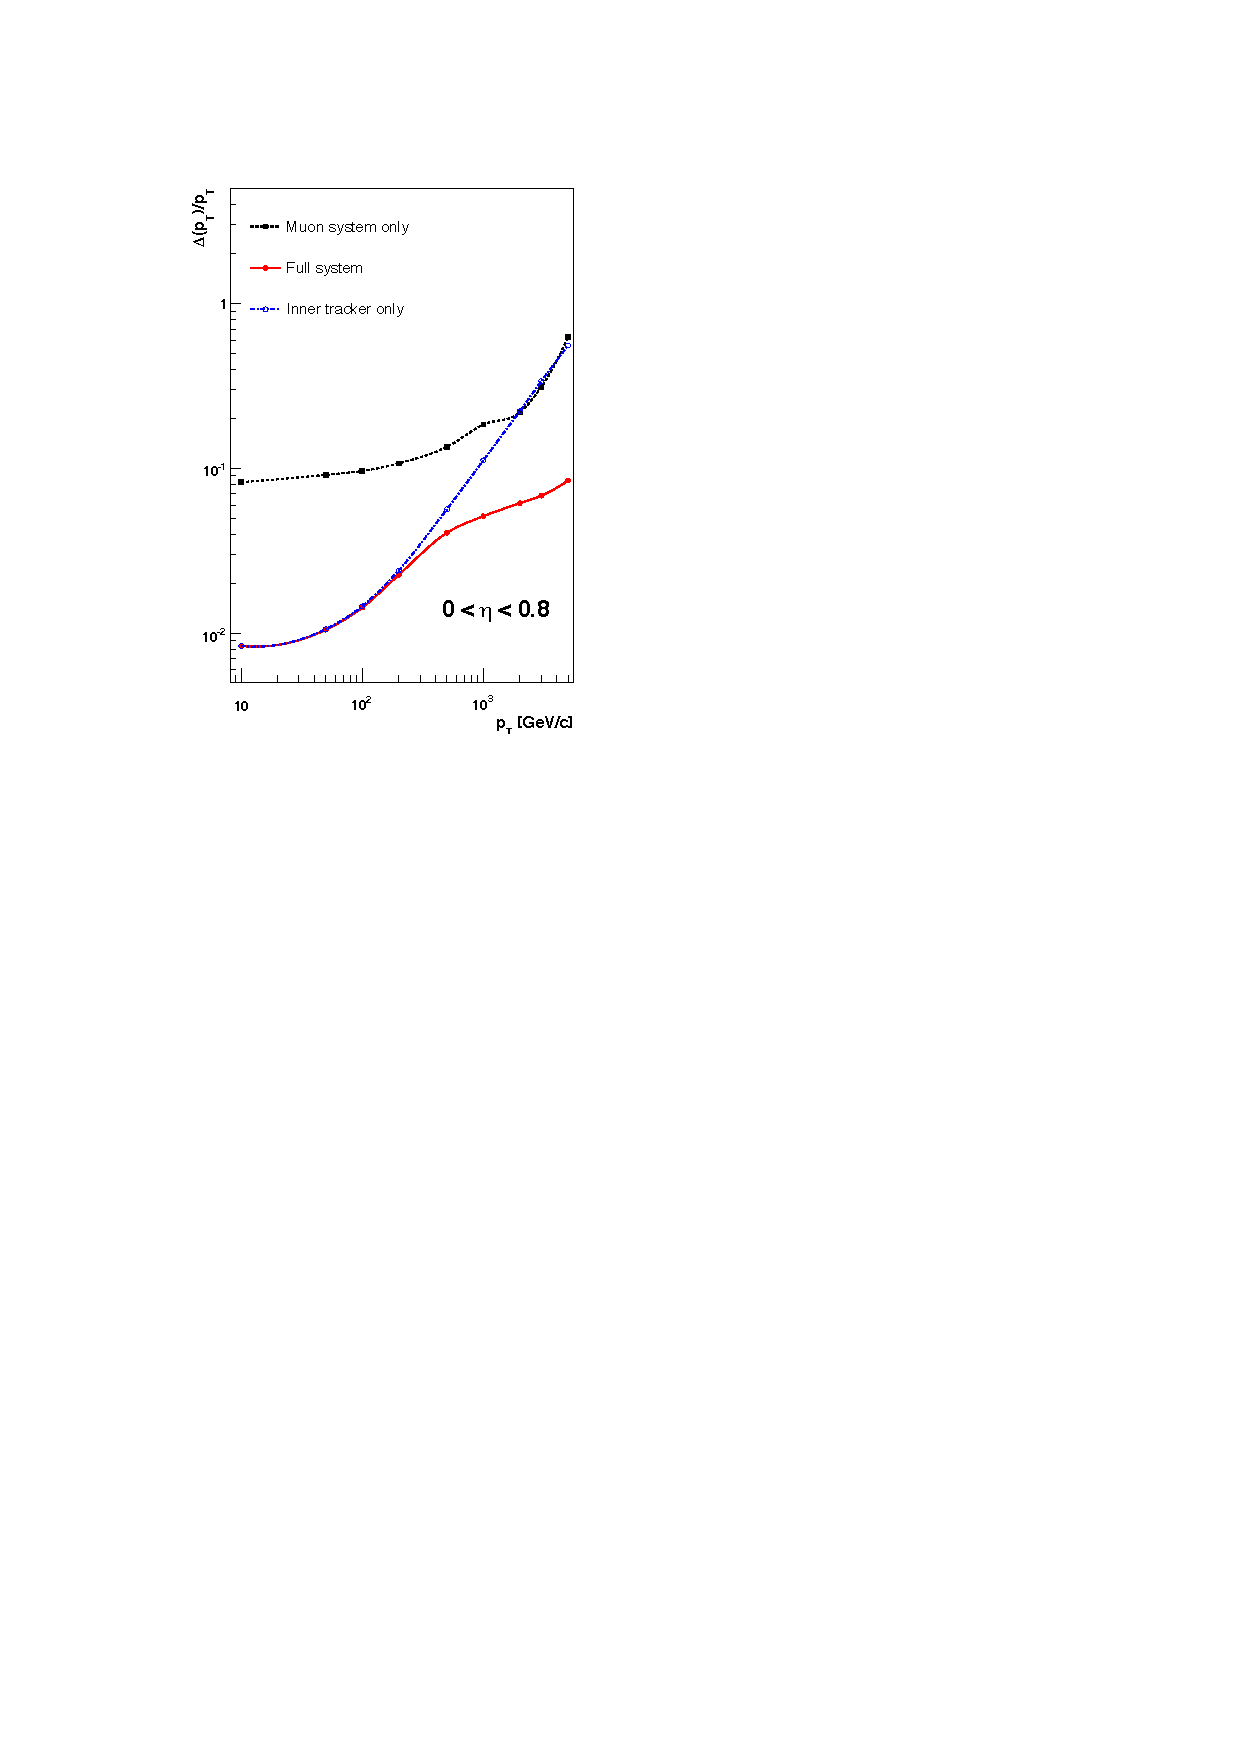
\includegraphics[height=0.4\textwidth]{ch2_cms_exp/plots/MuonResolution.pdf}
  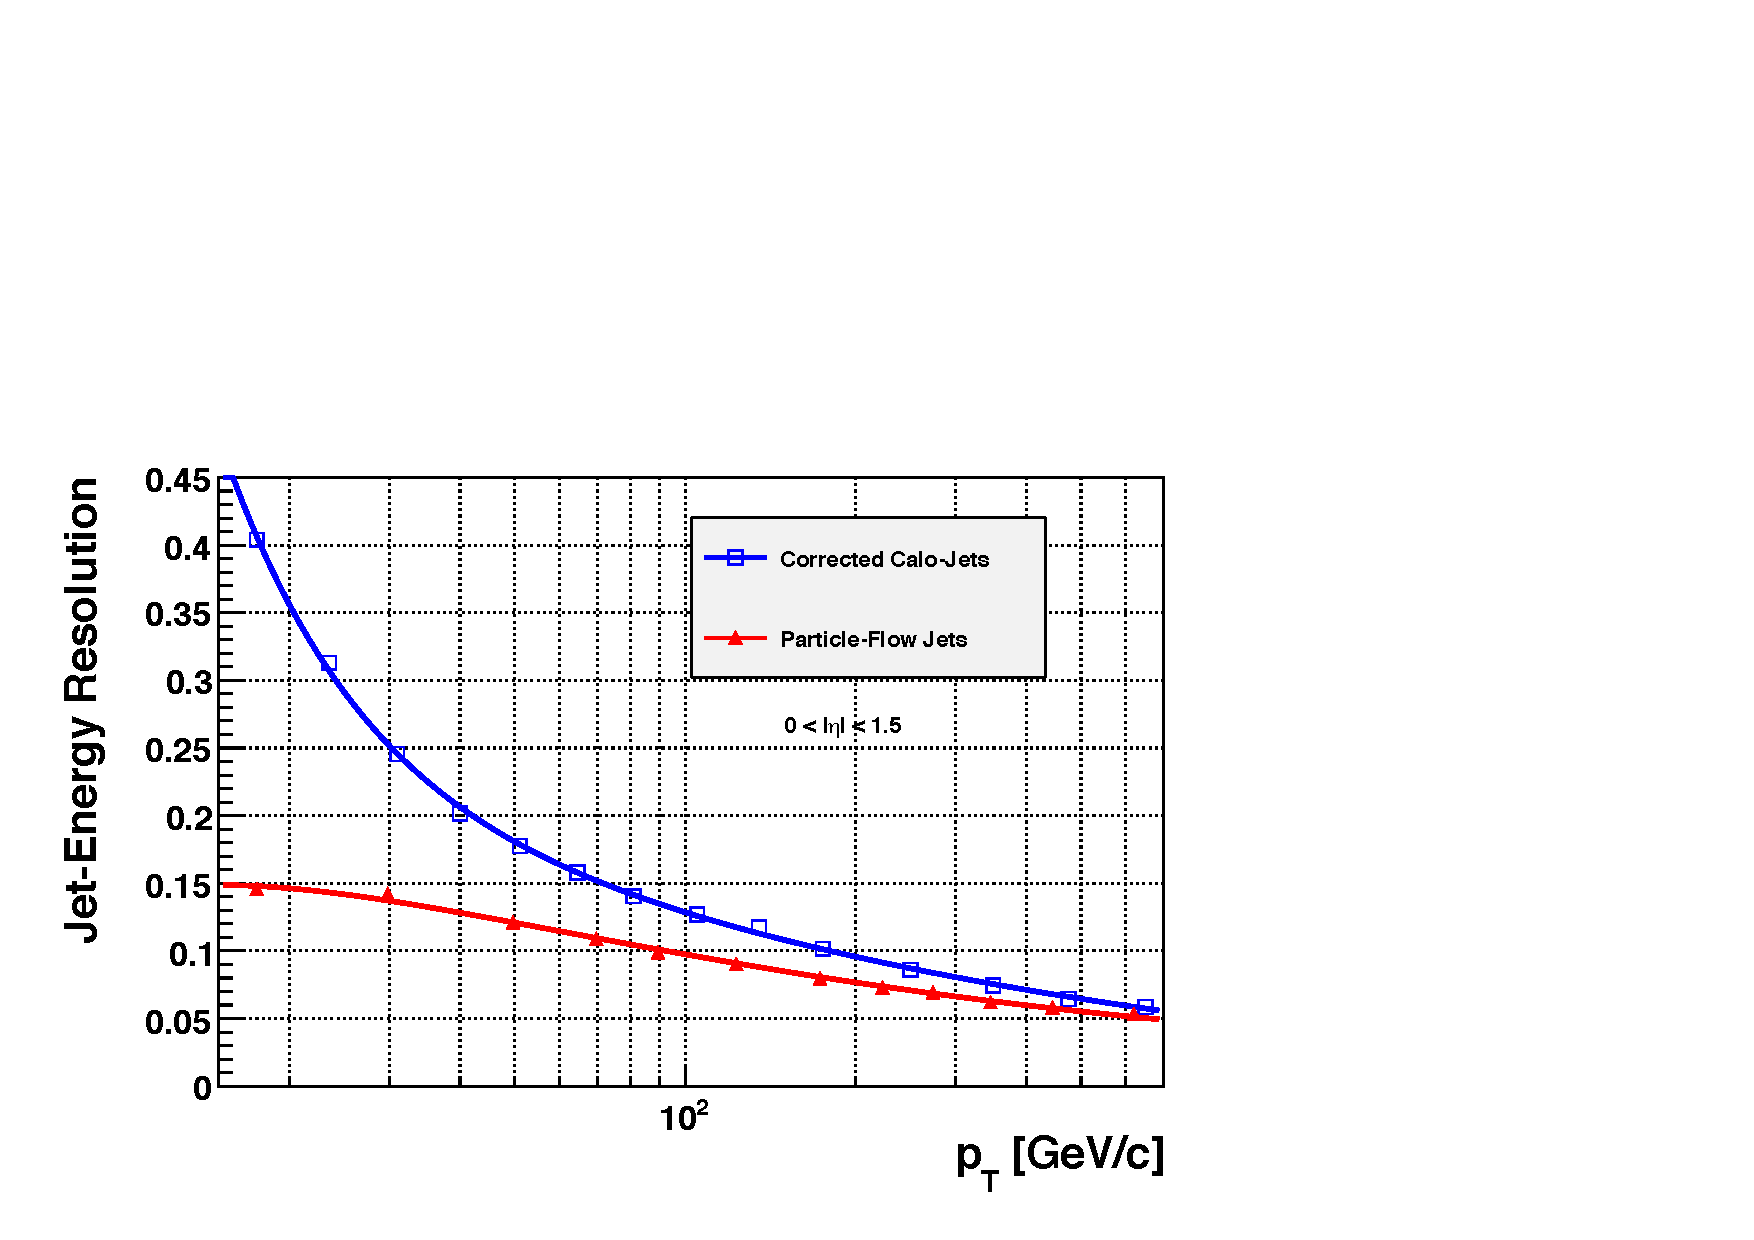
\includegraphics[height=0.4\textwidth]{ch2_cms_exp/plots/BarrelResolutionPFAndCalo.pdf}
  \caption[Particle flow jet resolution]{\textbf{Left:} The muon \pT resolution as a function of \pT for muons in the range $0<|\eta|<0.8$ when using only the muon system (black), only the tracking system (blue) and using both (red)~\cite{CMS_JINST}. \\ \textbf{Right:} The jet energy resolution as a function of jet \pT when using \PF jets as compared to calo jets~\cite{cms_pf_performance}.}
  \label{fig:muon_jet_res}
\end{figure}

\subsection{Isolation}
\label{sec:iso}

One way of differentiating between real (prompt) photons and fakes is the use of isolation. One would expect that in the absence of pileup a real photon would be isolated, which is to say there are no other particles (detector activity) in its vicinity. For a jet faking a photon (which is nearly always a \pizero) this is not the case and one would expect the \pizero to be surrounded by additional hadronised particles (detector activity in the tracker, \ECAL and \HCAL). In the \CMS \Hgg analysis isolation sums are used to distinguish prompt photons from fakes. Three variables are used which consider each photons isolation relative to activity in the surrounding environment. The procedure is to create a hollow cone around the photon candidate (of outer radius $\Delta R_{O}$ and inner radius $\Delta R_{I}$, where $\Delta R = \sqrt{\Delta\eta^{2}+\Delta\phi^{2}}$) and sum the energy contained in that cone of \PF candidates; charged hadrons, neutral hadrons and electrons/photons. These three variables are defined in the following way:

\begin{itemize}
  \item{\textbf{Charged hadron isolation:} Sum of charged hadron \PF candidates \ET in cone of $\Delta R_{O}=0.3$ and $\Delta R_{I}=0.02$.} 
  \item{\textbf{Neutral hadron isolation:} Sum of neutral hadron \PF candidates \ET in cone of $\Delta R_{O}=0.3$ and $\Delta R_{I}=0.0$.}
  \item{\textbf{$e/\gamma$ isolation:} Sum of $e/\gamma$ \PF candidates \ET in cone of $\Delta R_{O}=0.3$ with a central \eta strip of 0.070 (0.015) removed for barrel (endcap) photons.}
\end{itemize}

\subsection{Pileup}
\label{sec:pileup}

There can be up to $1.1\times10^{11}$ protons in each bunch at the \LHC which results in multiple interactions (can be as many as 50 primary vertices) per bunch crossing. This effect is known as pileup and can present a challenge in finding the primary vertex and also produces additional energy in each event which originates from somewhere other than the primary vertex. To combat the latter of these two effects a technique called $\rho$ subtraction is used to corrected the energy of jets and isolation sums for pileup. $\rho$ is defined as a per event quantity and is computed by summing the energy in all the calorimeters and dividing by the calorimeter area and thus represents the average energy density in the detector per event.




